\documentclass{beamer}
\usetheme{Warsaw}

\usepackage{polski}
\usepackage{tabularx}
\usepackage{listings}
\usepackage{color} %use color
\definecolor{mygreen}{rgb}{0,0.6,0}
\definecolor{mygray}{rgb}{0.5,0.5,0.5}
\definecolor{mymauve}{rgb}{0.58,0,0.82}

%Customize a bit the look
\lstset{ %
backgroundcolor=\color{white}, % choose the background color; you must add \usepackage{color} or \usepackage{xcolor}
basicstyle=\footnotesize, % the size of the fonts that are used for the code
breakatwhitespace=false, % sets if automatic breaks should only happen at whitespace
breaklines=true, % sets automatic line breaking
captionpos=b, % sets the caption-position to bottom
commentstyle=\color{mygreen}, % comment style
deletekeywords={...}, % if you want to delete keywords from the given language
escapeinside={\%*}{*)}, % if you want to add LaTeX within your code
extendedchars=true, % lets you use non-ASCII characters; for 8-bits encodings only, does not work with UTF-8
frame=single, % adds a frame around the code
keepspaces=true, % keeps spaces in text, useful for keeping indentation of code (possibly needs columns=flexible)
keywordstyle=\color{blue}, % keyword style
% language=Octave, % the language of the code
morekeywords={*,...}, % if you want to add more keywords to the set
numbers=left, % where to put the line-numbers; possible values are (none, left, right)
numbersep=5pt, % how far the line-numbers are from the code
numberstyle=\tiny\color{mygray}, % the style that is used for the line-numbers
rulecolor=\color{black}, % if not set, the frame-color may be changed on line-breaks within not-black text (e.g. comments (green here))
showspaces=false, % show spaces everywhere adding particular underscores; it overrides 'showstringspaces'
showstringspaces=false, % underline spaces within strings only
showtabs=false, % show tabs within strings adding particular underscores
stepnumber=1, % the step between two line-numbers. If it's 1, each line will be numbered
stringstyle=\color{mymauve}, % string literal style
tabsize=2, % sets default tabsize to 2 spaces
title=\lstname % show the filename of files included with \lstinputlisting; also try caption instead of title
}
%END of listing package%

\definecolor{darkgray}{rgb}{.4,.4,.4}
\definecolor{purple}{rgb}{0.65, 0.12, 0.82}

%define Javascript language
\lstdefinelanguage{TypeScript}{
keywords={typeof, new, true, false, catch, function, return, null, catch, switch, var, if, in, while, do, else, case, break, const},
keywordstyle=\color{blue}\bfseries,
ndkeywords={class, export, boolean, throw, implements, import, this},
ndkeywordstyle=\color{darkgray}\bfseries,
identifierstyle=\color{black},
sensitive=false,
comment=[l]{//},
morecomment=[s]{/*}{*/},
commentstyle=\color{purple}\ttfamily,
stringstyle=\color{red}\ttfamily,
morestring=[b]',
morestring=[b]"
}

\lstset{
language=TypeScript,
extendedchars=true,
basicstyle=\footnotesize\ttfamily,
showstringspaces=false,
showspaces=false,
numbers=left,
numberstyle=\footnotesize,
numbersep=9pt,
tabsize=2,
breaklines=true,
showtabs=false,
captionpos=b
}

\title{Angular}
\subtitle{Warsztaty}
\author{Piotr Wolny}
\institute{e-point SA}
\date{\today}

\begin{document}

\begin{frame}
    \titlepage
\end{frame}

\begin{frame}
    \frametitle{Wprowadzenie}
    \begin{itemize}
        \item AngularJS od 20xx roku
        \item Angular 2+ od 20xx roku
        \item TypeScript
    \end{itemize}
\end{frame}

\begin{frame}
    \frametitle{TypeScript}
    \begin{itemize}
        \item AngularJS od 20xx roku
        \item Angular 2+ od 20xx roku
        \item TypeScript
    \end{itemize}
\end{frame}

\begin{frame}
    \frametitle{Przegląd}
    \begin{itemize}
        \item Moduły
            \begin{itemize}
                \item grupują powiązane ze sobą elementy źródłowe
                \item aplikacja składa się z co najmniej 1 modułu (AppModule)
                \item mogą importować inne moduły
                \item klasa z dekoratorem @NgModule()
            \end{itemize}
        \item Komponenty
            \begin{itemize}
                \item widoki, z których składa się aplikacja
                \item klasa z dekoratorem @Component()
                \item szablon HTML i style CSS
            \end{itemize}
        \item Serwisy
            \begin{itemize}
                \item dostarczają funkcje niezwiązane bezpośrednio z warstwą widoku
                \item wstrzykiwanie zależnośaci
                \item klasa z dekoratorem @Injectable()
            \end{itemize}
    \end{itemize}
\end{frame}

\begin{frame}
    \frametitle{Przegląd}
    \begin{center}
	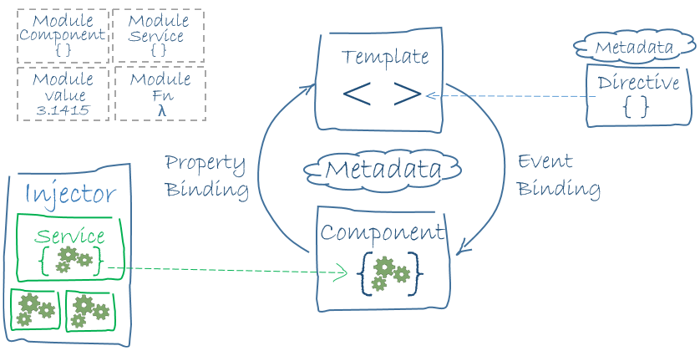
\includegraphics[scale=0.4]{overview2.png}
    \end{center}
\end{frame}

\begin{frame}
    \frametitle{Angular CLI}
    \begin{itemize}
        \item ng version (7.1.0!)
        \item ng new
        \item ng build --prod
        \item ng serve
        \item ng test
	\item ng lint
        \item ng generate
    \end{itemize}
\end{frame}

\begin{frame}
    \frametitle{Ćwiczenie 1: Angular CLI}
    \begin{itemize}
        \item Wygenerować nowy projekt ng-workshop (scss, ruting)
        \item Uruchomić aplikację
        \item Sprawdzić, czy działa pod adresem http://localhost:4200
        \item Uruchomić testy
	\item Uruchomić sprawdzanie stylu (ng lint)
        \item Zintegrować sprawdzanie stylu z IntelliJ IDEA
        \item Usunąć wygenerowaną zawartość szablonu (app.component.html)
        \item Wygenerować nowy komponent (header) z napisem ng-workshop
        \item Sprawdzić, czy aplikacja odświeżyła się automatycznie
    \end{itemize}
\end{frame}

\begin{frame}
    \frametitle{Struktura aplikacji}
    \begin{itemize}
        \item package.json
        \item angular.json
        \item src/index.html
        \item src/styles.scss
	\item src/app/app.module.ts
	\item src/app/app.component.ts
    \end{itemize}

    Najważniejsze katalog i pliki.
\end{frame}

\begin{frame}
    \frametitle{Ruting i nawigacja - podstawy}
    \begin{itemize}
        \item Moduł RouterModule (@angular/router)
        \item Dyrektywa <router-outlet>
        \item Dyrektywa <a routerLink="/jobs" routerLinkActive="active">Jobs</a>
        \item Serwis Router do nawigacji z kodu źródłowego: router.navigate(ByUrl)
    \end{itemize}
\end{frame}

\begin{frame}[fragile]
    \frametitle{Ruting - konfiguracja}
\begin{lstlisting}
const routes: Routes = [
  { path: '', component: HomepageComponent },
  { path: 'jobs', component: JobListComponent },
  { path: 'candidates', component: CandidateListComponent },
  { path: '**', component: PageNotFoundComponent },
];

@NgModule({
  imports: [RouterModule.forRoot(routes)],
  exports: [RouterModule]
})
export class AppRoutingModule { }
\end{lstlisting}
\end{frame}

\begin{frame}
    \frametitle{Ćwiczenie 2: Ruting}
    \begin{itemize}
        \item Wygenerować komponenty/strony:
	    \begin{itemize}
                \item homepage
		\item job-list
		\item candidate-list
		\item page-not-found
	    \end{itemize}
        \item Skonfigurować ruting: /, /jobs, /candidates i /**
        \item Dodać linki do nagłówka
    \end{itemize}
\end{frame}

\begin{frame}[fragile]
    \frametitle{Komponenty - definicja}
\begin{lstlisting}
@Component({
  selector:    'app-example',
  templateUrl: './example.component.html',
  styleUrls:   ['./example.component.scss']
  providers:   [ ExampleService ]
})
export class ExampleComponent implements OnInit {
/* . . . */
}
\end{lstlisting}
\end{frame}

\begin{frame}[fragile]
    \frametitle{Komponenty - szablon}
\begin{lstlisting}
<h2>Hero List</h2>

<p><i>Pick a hero from the list</i></p>
<ul>
  <li *ngFor="let hero of heroes" (click)="selectHero(hero)">
    {{hero.name}}
  </li>
</ul>

<app-hero-detail *ngIf="selectedHero" [hero]="selectedHero"></app-hero-detail>
\end{lstlisting}
\end{frame}

\begin{frame}
    \frametitle{Komponenty - drzewo}
    \begin{center}
	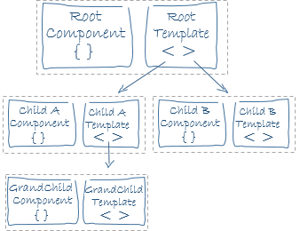
\includegraphics[scale=0.4]{component-tree.png}
    \end{center}
\end{frame}

\begin{frame}
    \frametitle{Komponenty - data binding}
    \begin{center}
	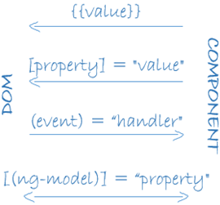
\includegraphics[scale=0.4]{databinding.png}
    \end{center}
\end{frame}

\begin{frame}
    \frametitle{Ćwiczenie 3: Wyświetlanie danych}
    \begin{itemize}
        \item Dodać klasę Job z polami code i name typu string
        \item Dodać tablicę jobs: Job[] do komponentu job-list
        \item Wyświetlić listę używająć dyrektywy *ngFor
    \end{itemize}
\end{frame}

\begin{frame}[fragile]
    \frametitle{Serwisy - definicja}
\begin{lstlisting}
@Injectable({ providedIn: 'root' })
export class ExampleService {
/* . . . */
}
\end{lstlisting}
\end{frame}

\begin{frame}
    \frametitle{Wstrzykiwanie zalezności}
    Hierarchiczny system injectorów. Konfiguracja:
    \begin{itemize}
        \item @Injectable({ providedIn: 'root' })
        \item @NgModule({ providers: [{ provide: LocationStrategy, useClass: HashLocationStrategy }] })
        \item @Component({ providers: [ ExampleService ]})
    \end{itemize}
\end{frame}

\begin{frame}
    \frametitle{Ćwiczenie 4: Pobieranie danych z serwisu}
    \begin{itemize}
        \item Dodać serwis JobService zwracający tablicę Job[]
        \item Dodać zależność od serwisu do komponentu JobListComponent
        \item Wypełnić tablicę jobs: Job[] danymi z serwisu
    \end{itemize}
\end{frame}

\begin{frame}
    \frametitle{Komunikacja z API HTTP}
    HttpClient z modułu HttpClientModule (@angular/common/http)
    \begin{itemize}
        \item Używamy w serwisach:
export class ExampleService {
  constructor(private http: HttpClient) { }
}
        \item Typujemy odpowiedź: this.http.get<DataType>(url)
        \item Zwraca Observable<DataType>
        \item this.http.post<DataType>(url, data)
    \end{itemize}
\end{frame}

\begin{frame}[fragile]
    \frametitle{Proxy do backendu}
    \tiny
    Ze względu na reguły CORS nie możemy wykonywać bezpośrednio żądań do API na innej domenie / innym porcie.
    Możemy skonfigurować lokalne proxy do API dodając plik src/proxy.conf.json:
\begin{lstlisting}
{
  "/api": {
    "target": "http://localhost:8080",
    "secure": false,
    "pathRewrite": {
      "^/api": ""
    }
  }
}
\end{lstlisting}
    I zmodyfikować angular.json:
\begin{lstlisting}
-            "browserTarget": "ng-workshop:build"
+            "browserTarget": "ng-workshop:build",
+            "proxyConfig": "src/proxy.conf.json"
\end{lstlisting}

\end{frame}

\begin{frame}
    \frametitle{Ćwiczenie 5: Pobieranie danych z serwisu}
    \begin{itemize}
        \item Zaimportować moduł HttpClientModule w AppModule
        \item Dodać zależność od HttpClient w JobService
        \item Skonfigurować proxy do API
        \item Pobrać dane z API (zwrócić uwagę na format JSON-a z API!)
    \end{itemize}
\end{frame}

\begin{frame}
    \frametitle{Reaktywne formularze}
    \begin{itemize}
        \item Definiowane przez model w komponencie: FormControl i FormGroup.
        \item FormBuilder do uproszczenia zapisu.
    \end{itemize}
\end{frame}

\begin{frame}[fragile]
    \frametitle{Ruting - zagnieżdżanie}
\begin{lstlisting}
const routes: Routes = [
  { path: '', component: HomepageComponent },
  { path: 'jobs', children: [
    { path: '', component: JobListComponent },
    { path: 'add', component: JobAddComponent },
  ]},
  { path: 'candidates', component: CandidateListComponent },
  { path: '**', component: PageNotFoundComponent },
];
\end{lstlisting}
\end{frame}

\begin{frame}
    \frametitle{Ćwiczenie 6: Użycie formularza do dodawania elementów}
    \begin{itemize}
        \item Zaimportować moduł ReactiveFormsModule w AppModule
        \item Dodać nowy komponent add-job
        \item Skonfigurować zagnieżdżony ruting do nowego komponentu
        \item Zdefiniować formularz w nowym komponencie
        \item Wysłać dane z formularza do API przez serwis
        \item Po udanym zapisaniu wrócić na ekran listy
    \end{itemize}
\end{frame}

\begin{frame}
    \frametitle{Ćwiczenie 6: Walidacja formularza}
    \begin{itemize}
    \end{itemize}
\end{frame}

\begin{frame}
    \frametitle{Komponenty - cykl życia}
\tiny
\begin{tabularx}{\textwidth}{l | X | X}
Metoda & Przeznaczenie & Wykonanie \\
\hline \hline
ngOnChanges() & Orzymuje obiekt SimpleChanges, zawierający aktualne i poprzednie wartości właściwości wejściowych. & Wywoływane przed ngOnInit() i przy każdej zmianie właściwości wejściowych (input properties).\\
ngOnInit() & Do inicjalizacji komponentu po ustawieniu właściwości wejściowych (input properties). & Wywoływane raz, po pierwszym ngOnChanges().\\
ngDoCheck() & Do wykrywania zmian, których Angular nie obsłuży automatycznie. & Wywoływane przy każdym przebiegu wykrywania zmian, zaraz po ngOnChanges() i ngOnInit().\\
ngAfterContentInit() & Respond after Angular projects external content into the component's view / the view that a directive is in. & Wywoływane raz, po pierwszym ngDoCheck().\\
ngAfterContentChecked()	& Respond after Angular checks the content projected into the directive/component. & Wywoływane po ngAfterContentInit() i każdym kolejnym ngDoCheck().\\
ngAfterViewInit() & Do działań po inicjalizacji widoku i widoków dzieci. & Wywoływane raz, po pierwszym ngAfterContentChecked().\\
ngAfterViewChecked() & Do działań po sprawdzeniu widoku i widoków dzieci. & Wywoływane po ngAfterViewInit i każdym kolejnym ngAfterContentChecked().\\
ngOnDestroy() & Do sprzątania przed zniszczeniem komponentu. Należy odsubskrybować Observable i odłączyć handlery zdarzeń. & Wywoływane przed zniszczeniem komponentu.\\
\end{tabularx}
\end{frame}

\begin{frame}
    \frametitle{Komponenty}
    \begin{itemize}
	\item Dyrektywy
	\item Pipe
        \item Angular material
    \end{itemize}
\end{frame}

\begin{frame}
    \frametitle{Moduły}
    \begin{itemize}
        \item declarations: The components, directives, and pipes that belong to this NgModule.
        \item exports: The subset of declarations that should be visible and usable in the component templates of other NgModules.
        \item imports: Other modules whose exported classes are needed by component templates declared in this NgModule.
        \item providers: Creators of services that this NgModule contributes to the global collection of services; they become accessible in all parts of the app. (You can also specify providers at the component level, which is often preferred.)
        \item bootstrap: The main application view, called the root component, which hosts all other app views. Only the root NgModule should set the bootstrap property.
    \end{itemize}
\end{frame}

\end{document}
